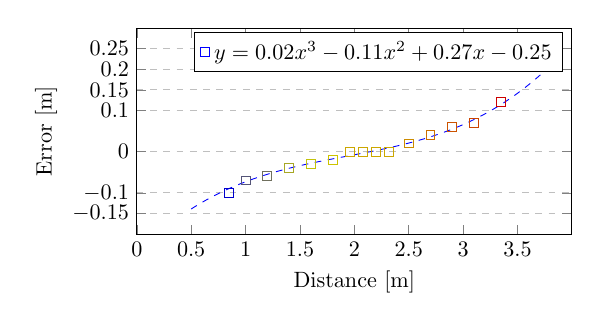
\begin{tikzpicture}[scale=0.8]
	\begin{axis}[
			xlabel={Distance [m]},
			ylabel={Error [m]},
			xmin=0, xmax=4,
			ymin=-0.2, ymax=0.3,
			xtick={0,0.5,1,1.5,2,2.5,3,3.5},
			ytick={-0.15,-0.1,-0.5,0,0.5,0.1,0.15,0.2,0.25},
			ymajorgrids=true,
			grid style=dashed,
			height=0.4\textwidth,
			width=0.7\textwidth,
		]
																																									
		\addplot+[
			only marks,
			scatter,
			color=blue,
			mark=square,
		]
		coordinates {
			(0.85,-0.10)(1.00,-0.07)(1.20,-0.06)(1.40,-0.04)(1.60,-0.03)(1.80,-0.02)(1.96, 0.00)(2.08, 0.00)(2.20, 0.00)(2.32, 0.00)(2.50, 0.02)(2.70, 0.04)(2.90, 0.06)(3.10, 0.07)(3.35, 0.12)
		};
																																									
		\addplot [
			dashed,
			domain=0.5:3.8, 
			samples=100, 
			color=blue,
		]
		{0.0194*x^3 - 0.1125*x^2 + 0.2672*x - 0.2472};
		\legend{$y = 0.02x^3 - 0.11x^2 + 0.27x - 0.25$}
	\end{axis}
\end{tikzpicture}	